% IPEC2026.cls is based on IEEEtran.cls.
% Please read the instructions for IEEEtran.cls before using IPEC2026.cls.
\newcommand{\CLASSINPUTtoptextmargin}{1.9cm}
\newcommand{\CLASSINPUTbottomtextmargin}{2.54cm}
\documentclass[a4paper]{IPEC2026}
%\usepackage[left=1.6cm,right=1.6cm,top=1.9cm,bottom=2.54cm]{geometry}
%\IEEEoverridecommandlockouts
% The preceding line is only needed to identify funding in the first footnote. If that is unneeded, please comment it out.
\usepackage{cite}
\usepackage{amsmath,amssymb,amsfonts}
\usepackage{algorithmic}
\usepackage{graphicx}
\usepackage{textcomp}
\usepackage{xcolor}
\usepackage{url} 
\def\BibTeX{{\rm B\kern-.05em{\sc i\kern-.025em b}\kern-.08em
    T\kern-.1667em\lower.7ex\hbox{E}\kern-.125emX}}
\usepackage{pgfplots}
\pgfplotsset{compat=1.18}
\usepackage[font={footnotesize}]{caption}          % Necessary for subcaption
\usepackage{subcaption}       % Multiple figures in one
\usepackage{tabularx}
\usepackage{tabularray}
\UseTblrLibrary{booktabs}

\usepackage{siunitx}                % Units; e.g. prevents linebreak between number and unit
\sisetup{
  per-mode=symbol-or-fraction,
  output-exponent-marker=\ensuremath{\mathrm{e}},
  %range-units = single  % Use 1 to 3 MHz instead of 1 MHz to 3 MHz
  %fraction-function=\tfrac
}
\DeclareSIUnit{\inch}{in}

% Adjust the spacing around a figure
% 8pt plus 1pt minus 2pt: a “rubber length” with base = 8pt; stretch = up to +1pt (can grow to 9pt if there’s extra space); shrink = up to −2pt (can shrink to 6pt if the page is tight)
%\setlength{\textfloatsep}{5pt plus 3pt minus 1pt}    
% Space above/below display equations
%\setlength{\abovedisplayskip}{7pt plus 3pt minus 1pt}  
%\setlength{\belowdisplayskip}{7pt plus 3pt minus 1pt} 
% “Short” variants used when the preceding line is short or ends with a display trigger
%\setlength{\abovedisplayshortskip}{6pt plus 3pt minus 1pt}
%\setlength{\belowdisplayshortskip}{6pt plus 3pt minus 1pt}

\usepackage[acronym]{glossaries}
% Just for having less to type
\newcommand{\sbl}[1]{\glssymbol{#1}}
% To allow compatibility with acronym package syntax, define \ac
\newcommand{\ac}{\gls}
\newcommand{\acp}{\glspl}

\newcommand{\mathSymbol}[3]{
    \newglossaryentry{#1}{symbol={\ensuremath{#2}}, name={#3}, description={}, sort={#1}}
}

\mathSymbol{Lself}{L_\mathrm {self}}{Self-inductance of each coil of a symmetrical coupled inductor}
\mathSymbol{k}{k}{Coupling-factor of the coupled inductor}
\mathSymbol{Lm}{L_\mathrm m}{Magnetizing inductance in the transformer model}
\mathSymbol{Lout}{L_\mathrm {out}}{Output inductance in the transformer model}
\mathSymbol{im}{i_\mathrm m}{Magnetizing current in the transformer model}
\mathSymbol{iout}{i_\mathrm {out}}{Output current}
\mathSymbol{iout_avg}{\overline{i_\mathrm {out}}}{Average output current}
\mathSymbol{v1}{v_\mathrm 1}{Voltage at the switch-node leg 1}
\mathSymbol{v2}{v_\mathrm 2}{Voltage at the switch-node leg 2}
\mathSymbol{i1}{i_\mathrm 1}{Current of leg 1}
\mathSymbol{i2}{i_\mathrm 2}{Current of leg 2}
\mathSymbol{vout}{v_\mathrm {out}}{Output voltage}
\mathSymbol{Ts}{T_\mathrm s}{Switching period}
\mathSymbol{fs}{f_\mathrm s}{Switching frequency}
\mathSymbol{Deff}{D_\mathrm {eff}}{Effective duty cycle}
\mathSymbol{D}{D}{Duty cycle}
\mathSymbol{Vin}{V_\mathrm {in}}{Input voltage}
\mathSymbol{DeltaIleg}{\Delta I_\mathrm {leg}}{Peak-to-peak leg current ripple}
\mathSymbol{DeltaIout}{\Delta I_\mathrm {out}}{Peak-to-peak output current ripple}
\mathSymbol{Ion}{I_\mathrm {on}}{Turn-on current}
\mathSymbol{Ion,max}{I_\mathrm {on,max}}{Maximum turn-on current}
\mathSymbol{Hdc}{H_\mathrm {dc}}{DC field strength}
\mathSymbol{mui}{\mu _\mathrm i}{Initial Permeability}
\mathSymbol{Pout}{P_\mathrm {out}}{Output Power}
\mathSymbol{Cin}{C_\mathrm {in}}{Input capacitance}
\mathSymbol{Cout}{C_\mathrm {out}}{Output capacitance}

\newacronym{tcm}{TCM}{triangular current mode}
\newacronym{zvs}{ZVS}{zero voltage switching}
\newacronym{pcb}{PCB}{printed circuit board}
\newacronym{gan}{GaN}{Gallium Nitride}

\begin{document}

\title{Compact Single-Turn Coupled Inductor for MHz-Range Buck Converters with Zero Voltage Switching}
\track{6. Vehicle Electrification-related Technologies}
%Class IPEC2026: The \author command is disabled in this template.

\maketitle

\begin{abstract}
The next generation of automotive vehicles and datacenters requires highly compact and efficient 48~V to 12~V point-of-load converters. This paper presents a novel single-turn planar inductor geometry with four poles and dual air gap for operation beyond 1~MHz that minimizes copper-losses from external proximity effect. An experimental prototype with 1~kW output achieves a power density of 80~kW/L (1300~W/in³) and a peak efficiency of 96.3\%, demonstrating the potential of the inductor structure.
\end{abstract}

\begin{IEEEkeywords}
automotive 48 V to 12 V, coupled inductor, high power density, soft-switching
%The authors shall provide up to 4 keywords or phrases (in alphabetical order and separated by commas) to help identify the major topics of the paper.
\end{IEEEkeywords}

\section{Introduction}
With a growing power demand, power distribution in both conventional and electric vehicles presents an increasing challenge. Traditionally, \qty{12}{\V} are used to distribute the power to all auxiliary devices which requires large cable diameters. Moving to a \qty{48}{\V} distribution bus reduces the cost of the wire assembly and losses \cite{kumawatComprehensiveStudyAutomotive2019}. As devices with lower power consumption are still operating at \qty{12}{\V}, highly compact and efficient point-of-load converters are required. This conversion stage is a critical part of distributed power architectures and its performance has a direct impact on system-level efficiency, thermal design, and overall build volume \cite{kumawatComprehensiveStudyAutomotive2019}. With the rise of \ac{gan} power devices, operating converters in the MHz-range has become feasible, significantly reducing their size \cite{weitzHighFrequencyResonant2023}. 
At these frequencies, using planar magnetics with \ac{pcb} windings is beneficial as they allow elaborate winding structures, direct integration with the other circuitry, and efficient cooling due to their large surface area \cite{wangPCBWindingBasedCoupled2023, liHighFrequencyHigh2018, schaferNovelHighlyEfficient2020, caiOptimalDesignMegahertz2020}. 
%At these frequencies, the small number of turns permits the use of planar magnetics with \ac{pcb} windings, which allow elaborate winding structures, direct integration with the other circuitry, and efficient cooling due to their large surface area.
%As a low number of turns is required at these frequencies, planar magnetics that use \ac{pcb} windings can be used. This allows elaborate winding structures, effective cooling due to the large area per volume and direct integration with the other circuitry
Resonant converters with fixed gain based on planar transformers are a common choice for \qtyrange{48}{12}{\V} conversion but they are unsuitable when a regulated output voltage is required over a wide input voltage range. In these cases, the classical buck converter is appropriate but the design of compact and efficient planar inductors is challenging due to the missing possibility for interleaving, the fringing effect of the air gap, and the DC-bias in the core. \par

In this paper, a \qty{1}{\kW} 2-phase coupled inductor buck converter for \qtyrange{48}{12}{\V} conversion is studied. To minimize the overall volume, a target switching-frequency range of \qtyrange{1}{3}{\MHz} was selected. Compared to previous work \cite{nan1MHzBidirectional2016, dongInvestigationMultiphaseCoupledInductor2009, shaZVSInterleavedSynchronousBuck2022, huaUltrathinCoupledInductor2021, wangPCBWindingBasedCoupled2023}, the low operating voltage requires a very low inductance whose design becomes particularly challenging due to the large phase current of \qty{40}{\A} with \qty{100}{\A} of ripple (required to achieve soft-switching). Firstly, the effects of coupling on the electrical parameters are analyzed mathematically. Afterwards, different geometries for the single-turn inductor are optimized using a novel winding geometry and dual air gaps. The most promising geometry based on the four-pole structure is implemented and tested in an experimental prototype. 

\pagebreak

\section{Coupled inductor buck converter in TCM}
\paragraph{Working principle}
\begin{figure}
  \centering
  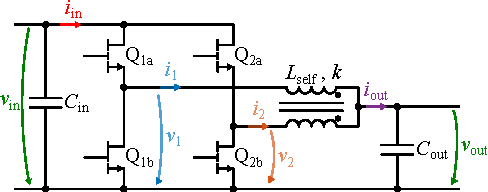
\includegraphics[width=0.9\columnwidth]{../figures/Inkscape/Schematic.pdf}
  \caption{Schematic of the Coupled Inductor Buck Converter.}
  \label{fig:Schematic_BuckConfig_Coupled}
\end{figure}

\begin{figure}
  \begin{subfigure}[c]{0.51\columnwidth}
      \centering
      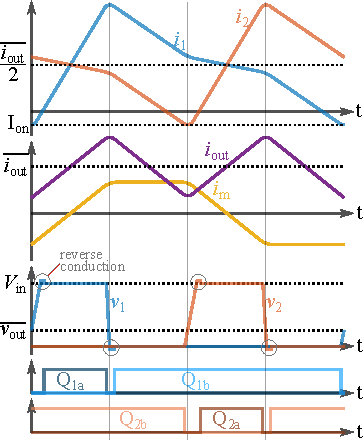
\includegraphics[width=\textwidth]{../figures/Inkscape/Waveforms_negative.pdf}
      \subcaption{Negative Coupling}
      \label{fig:waveform_negCoupling}
    \end{subfigure}
    \begin{subfigure}[c]{0.48\columnwidth}
      \centering
      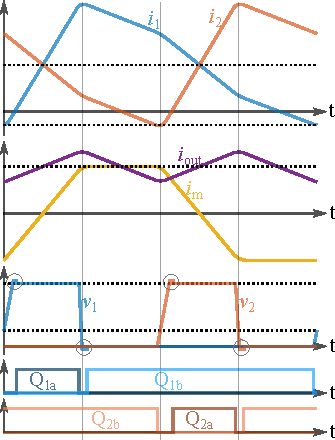
\includegraphics[width=\textwidth]{../figures/Inkscape/Waveforms_positive.pdf}
      \subcaption{Positive Coupling}
      \label{fig:waveform_posCoupling}
    \end{subfigure}
  \caption{Waveforms for positive and negative coupling; dead-times are exaggerated. It can be seen that the slopes are changed but the behavior in the vicinity of the switching instances is fundamentally the same.}
  \label{fig:waveform_Coupling}
\end{figure}
The topology of the two phase coupled-inductor buck converter is shown in Fig. \ref{fig:Schematic_BuckConfig_Coupled}. It operates like a conventional two-phase buck with both legs switched \qty{180}{\degree} out of phase. When leg 2 is pulled high, the current in leg 1 is also affected as shown in Fig. \ref{fig:waveform_Coupling}. For positive coupling, the falling slope is steepened while for negative coupling it is flattened. 
Operation in \ac{tcm} enables \ac{zvs} by increasing the phase current ripple to more than two times the average phase current (Fig. \ref{fig:waveform_Coupling}) \cite{henzeZerovoltageSwitchingHigh1988}. The low-side switch is kept on after the zero-crossing of the leg current for a short period of time such that the current becomes negative. Once the low-side switch is disabled, the inductor current charges/discharges the GaN-FETs' drain-source capacitances until the high-side GaN-FET enters reverse conduction. High losses are observed during reverse conduction requiring precise dead-time calculation and adaptive switching frequency \cite{haiderAnalyticalCalculationResidual2021}. Turn-off losses remain but are small due to the large drain-source capacitance. 

\paragraph{Impact of the Coupling Factor}
\begin{figure}
  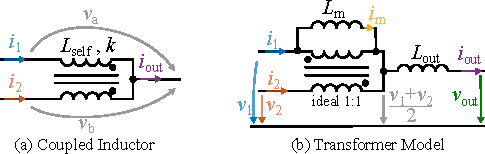
\includegraphics[width=0.9\columnwidth]{../figures/Inkscape/Transformer-Model.pdf}
  \caption{The coupled inductor can be described with a self-inductance \sbl{Lself} and coupling factor \sbl{k} or by using an equivalent circuit consisting of an ideal 1:1 transformer with magnetizing inductance \sbl{Lm} and common output inductance \sbl{Lout}.}
  \label{fig:InductorModel}
\end{figure}
The symmetrical coupled inductor consists of two identical coils. They are wound in a way, that the flux of one coil links with the flux of the second coil and vice versa with both coils connected on one side. This can be described mathematically using 
\begin{equation}
  \label{eq:StandardCoupling}
  \begin{bmatrix} v_\mathrm a \\ v_\mathrm b \end{bmatrix} = \begin{bmatrix} 1 & \sbl{k} \\ \sbl{k} & 1 \end{bmatrix} \sbl{Lself} \begin{bmatrix} \frac{d\sbl{i1}}{dt}  \\ \frac{d\sbl{i2}}{dt} \end{bmatrix}
\end{equation}
with self-inductance \sbl{Lself} and magnetic coupling-factor \sbl{k} ($-1 \leq k \leq 1$).
In order to provide a more intuitive understanding, the equivalent circuit in Fig. \ref{fig:InductorModel} (b) is introduced. Both circuits are electrically equivalent for $\sbl{Lout} = (1+\sbl{k})\frac{\sbl{Lself}}{2}$ and $\sbl{Lm} = (1-\sbl{k})\frac{\sbl{Lself}}{2}$.
The voltage at the virtual central node in the transformer model is only dependent on the two leg voltages \sbl{v1} and \sbl{v2}, decoupling the governing equations:
\begin{equation}
  \label{eq:TransformerModel}
  \begin{aligned}
    \frac{d\sbl{iout}}{dt} &= \frac{1}{\sbl{Lout}} \left (\frac{\sbl{v1} + \sbl{v2}}{2}-\sbl{vout} \right ) \\
    \frac{d\sbl{im}}{dt} &= \frac{1}{\sbl{Lout}} \left (\frac{\sbl{v1} - \sbl{v2}}{2} \right ) \\
    \text{with} \quad \sbl{iout} &= \sbl{i1} + \sbl{i2} \quad \text{and} \quad \sbl{im} = \sbl{i1} - \sbl{i2}
  \end{aligned}
\end{equation}
From this, the differential equations for each interval can be easily calculated and equations for the important converter parameters can be derived. An effective duty cycle \sbl{Deff} is introduced with $\sbl{Deff} = D$ for $\sbl{D} \leq 0.5$ and $\sbl{Deff} = 1-D$ for $\sbl{D} > 0.5$ to create universal equations. The peak-to-peak output ripple is then given by
\begin{equation}
  \sbl{DeltaIout} = \frac{2\sbl{Vin}}{\sbl{fs}(1+\sbl{k})\sbl{Lself}}\sbl{Deff}\left (\frac{1}{2}-\sbl{Deff} \right ).
  \label{eq:DeltaIout}
\end{equation}
The peak-to-peak ripple in each leg which is important for soft-switching is
\begin{equation}
  \sbl{DeltaIleg} =  \frac{\sbl{Vin}\sbl{Deff}}{2\sbl{fs}\sbl{Lself}} \left (\frac{2}{1+\sbl{k}} \left (\frac{1}{2}-\sbl{Deff} \right ) + \frac{1}{1-\sbl{k}} \right ).
  \label{eq:DeltaIleg}
\end{equation}

\sbl{Ion} needs to be below a certain negative value \sbl{Ion,max} to guarantee a sufficiently short dead time. This is fulfilled for
\begin{equation}
    \sbl{fs} < \frac{\sbl{Vin}\sbl{Deff}}{2\sbl{Lself}(\sbl{iout_avg}+2\sbl{Ion,max})} \left (\frac{2}{1+\sbl{k}}\left (\frac{1}{2}-\sbl{Deff} \right ) + \frac{1}{1-\sbl{k}} \right )
    \label{eq:ConditionZVS}
\end{equation}
where \sbl{iout_avg} is the average value of \sbl{iout}.

\section{Inductor Design}
\paragraph{Inductor geometry}
\begin{figure}
  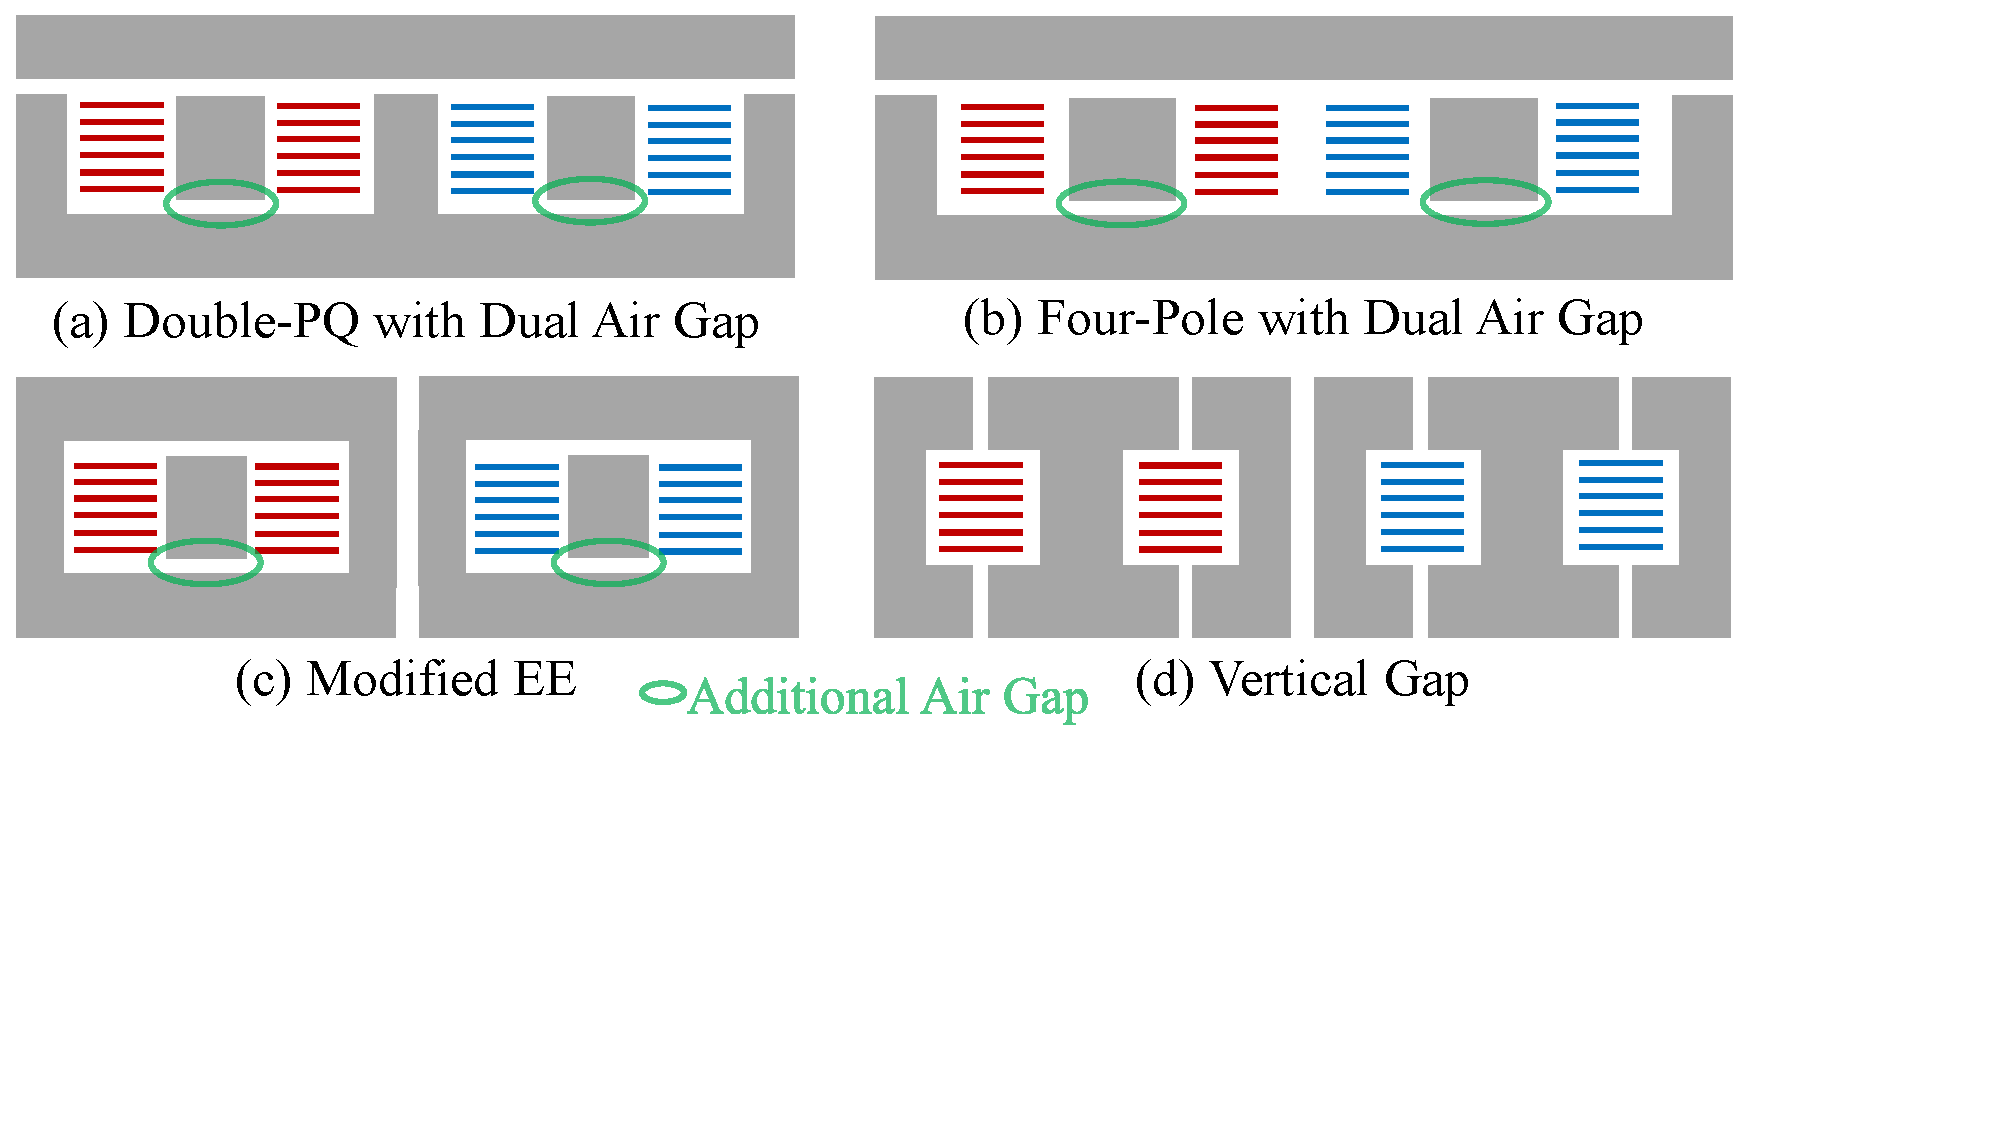
\includegraphics[page=1, trim = 0cm 6.8cm 4.5cm 0cm, clip, width=\columnwidth]{../figures/IPEC_Figures_PowerPoint.pdf}
  \caption{Structure of the studied cores in side-view if cut through the middle. First winding in red, second winding in blue.}
  \label{fig:Core_Drawings}
\end{figure}
This work introduces an additional air-gap to different designs as shown in Fig. \ref{fig:Core_Drawings}. Four geometries, two coupled, and two uncoupled ones, were compared: The Double-PQ structure (Fig. \ref{fig:Core_Drawings} (a)) was originally introduced by \cite{wangPCBWindingBasedCoupled2023} and combines two EQ-cores placed next to each other. The four-pole structure (Fig. \ref{fig:Core_Drawings} (b)) is very similar but omits the central pole \cite{huaUltrathinCoupledInductor2021}. Both of these geometries were originally constructed with two pieces such that there is only an air gap at the top.
The third geometry (Fig. \ref{fig:Core_Drawings} (c)) is basically an EE-Core but instead of one central gap, two gaps are used. Lastly, the vertical gap geometry (Fig. \ref{fig:Core_Drawings} (d)) proposed by \cite{schaferNovelHighlyEfficient2020} is investigated. The vertical air gap creates a fringing field in the middle of the windings. This partly compensates the internal proximity effect and draws current to the center, reducing losses. The main downside of this design is the significant external field on top and bottom of the inductor, making cooling difficult as no conductive material can be placed on top or bottom of the core. \par

All designs use a single turn with all six layers in parallel, significantly differing from the original designs. Designs with more than one turn were not considered because the desired inductance and coupling-factor could not be achieved in that case due to fringing and flux leakage between the pillars.

\paragraph{Material limitations}
TDK's PC200 was selected for this design as it exhibits very low loss in the range of \qtyrange{1}{4}{\MHz}. However, the performance of PC200 significantly degrades for a field strength $\sbl{Hdc} > \qty{50}{\A\per\m}$ and at $\sbl{Hdc} > \qty{100}{\A\per\m}$ its losses double \cite{tdkHighFrequencyLowLossFerrite}. Therefore, the inductor was designed with a maximum \sbl{Hdc} of \qty{40}{\A\per\m} to have some margin.

\paragraph{Positive vs negative coupling}
\begin{figure}
    \centering
    %\resizebox{0.9\columnwidth}{!}{\input{../figures/Python/current_ripple_plot.pgf}}
    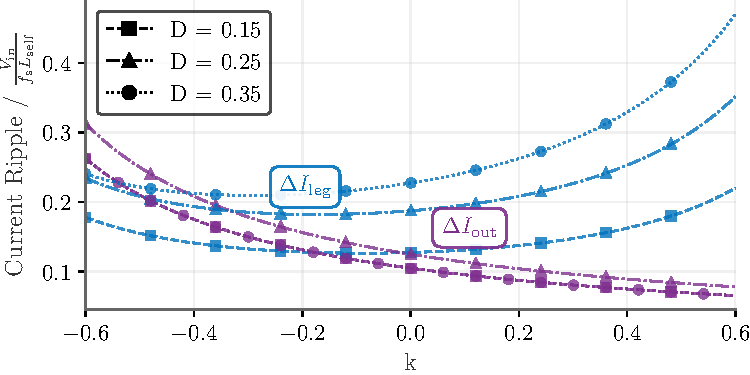
\includegraphics[width=0.95\columnwidth]{../figures/Python/current_ripple_plot.pdf}
    \caption{Peak-to-peak leg and output current ripple in dependency of the coupling factor for different duty cycles \sbl{D}. \textit{Note:} For $\sbl{D}=0.15$ and $\sbl{D}=0.35$ the output current ripple is identical so the curves overlap.}
    \label{fig:OutputAndLegRipple}
\end{figure}
\begin{figure}
  \includegraphics[page=3, trim = 0cm 1cm 3.5cm 0cm, clip, width=\columnwidth]{../figures/IPEC_Figures_PowerPoint.pdf}
  \caption{Flux-Distribution for negative and positive coupling of otherwise identical designs for a DC phase current of \qty{40}{\A} and \qty{100}{\A} of ripple.}
  \label{fig:Fluxposneg}
\end{figure}

Equation (\ref{eq:DeltaIout}) and (\ref{eq:DeltaIleg}) are plotted in Fig. \ref{fig:OutputAndLegRipple} for positive and negative coupling-factors. While a strong positive coupling decreases \sbl{DeltaIout} it increases \sbl{DeltaIleg}.
Overall, positive coupling is slightly beneficial from an electrical point of view as it reduces the output ripple. The higher \sbl{DeltaIleg} requires a larger \sbl{Lself} resulting in even lower \sbl{DeltaIout}. However, there is a very notable difference in the flux distribution as shown in Fig. \ref{fig:Fluxposneg}: For negative coupling, the two windings generate an opposing magnetomotive force at DC, resulting in a low flux that circulates through the outer air gaps. For positive coupling, the two magnetomotive forces are driving a DC-flux in the same direction causing a large flux that only circulates between the two windings where the reluctance is much lower. The peak flux-density is almost three times larger for positive coupling and as the core should be designed with respect to the \sbl{Hdc} limit, this means thicker top and bottom areas would be needed. Therefore, negative coupling is selected for this application\footnote{Note that for lower frequency materials which are less affected by DC flux, the picture would change: Those designs would likely benefit from positive coupling as the flux-density at the fundamental is reduced.}. 

\paragraph{Simulation Process}
For the simulation, the open-source 2D FEM software FEMM was used due to its high speed and easy integration with Matlab. As the core-structures are neither planar nor axisymmetric, the designs were first transformed to a planar structure. All cross-sectional areas are kept the same and the depth of the design is determined by the length of the winding. 

\paragraph{Split air gap and optimized windings}
\begin{figure}
  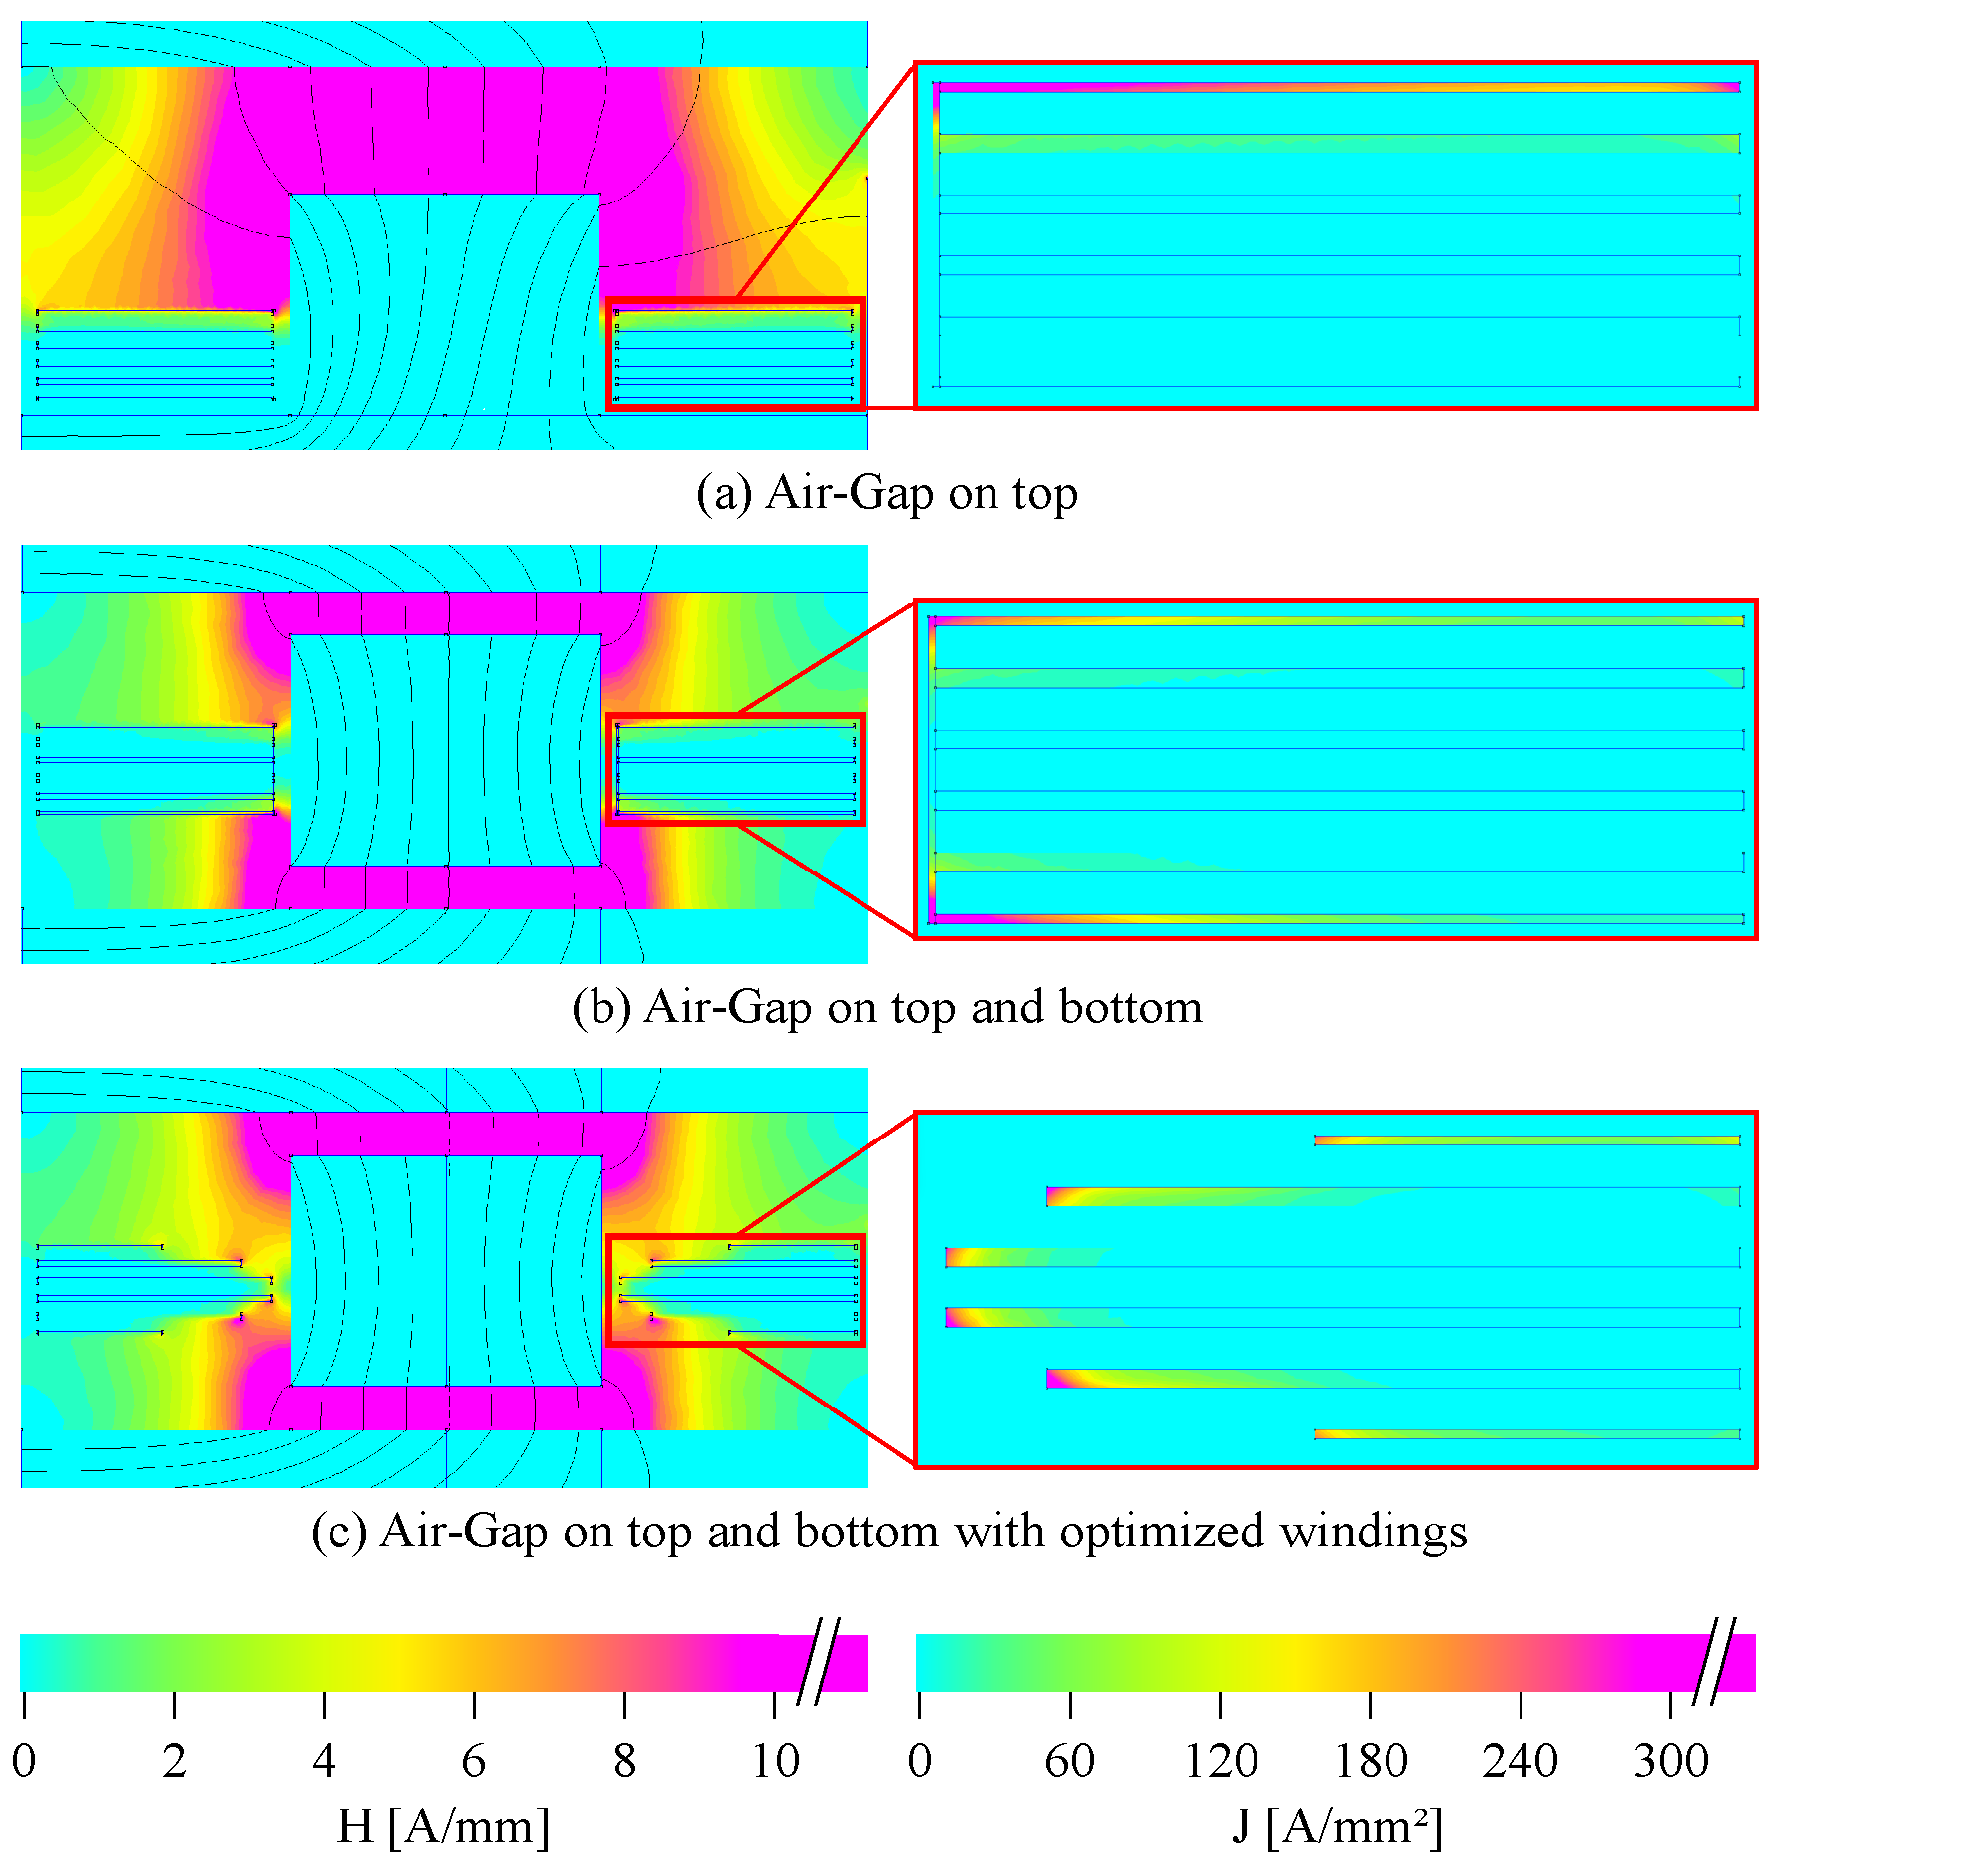
\includegraphics[page=1, trim = 0cm 0cm 3cm 0cm, clip, width=\columnwidth]{../figures/IPEC_Figure_AirGap.pdf}
  \caption{Field and current distribution for different approaches. Because all layers are in parallel the current crowds in areas of large field-strength. By splitting the gap, the field gets distributed more evenly and the current distribution improves. Utilizing a smaller width for the outer layers, i.e. moving the copper away from the high-flux areas distributes the current even better.}
  \label{fig:OptimizedGap}
\end{figure}

\begin{table}
  \caption{Comparison of the size and loss of the optimized pillar and windings for the four-pole design.}
  \label{tab:OptimizationPQ}
  \centering
  \begin{tblr}{
      colspec={Xll},
      row{1}={font=\bfseries},
      column{1}={font=\itshape},
      row{even}={bg=gray!10},
    }
    & {Volume [\unit{\cubic\cm}]} & {Copper Loss [\unit{\W}]} \\
    \toprule
    Original design & 5.8 & 7.0 \\
    Air gap on top and bottom & 5.5 & 5.7 \\
    Air gap on top and bottom, curved windings & 5.3 & 5.0 \\
    \bottomrule
  \end{tblr}
\end{table}

The external proximity effect caused by the air gap plays an important role for the current distribution and consequently the losses of this high-frequency inductor. The field-strength at the top of the windings is large and almost zero at the bottom. As a result, the AC current is only flowing in the top layers. By centering the pillar vertically in the window such that there is an equal air gap on the top and on the bottom, the field-strength is distributed much more uniformly and current flows in the top and bottom layers. This results in a \qty{20}{\percent} reduction in losses, which can be reduced even further by using curved windings as shown in Table \ref{tab:OptimizationPQ}.

\paragraph{Comparison of Core Structures}
Table \ref{tab:InductorComparison} compares the different core structures for a design with $\sbl{fs}=\qty{1.5}{\MHz}$ at $\sbl{iout_avg} = \qty{80}{\A}$ and $\sbl{k} = -0.3$. This coupling factor was chosen because it allows the use of small air gaps at the pillar which reduces copper losses due to the smaller external field while still not increasing \sbl{DeltaIout} too much. The cross-sectional areas were designed to result in $\sbl{Hdc} \leq \qty{40}{\A\per\m}$. All designs except the one with vertical gap use the optimized curved windings. The four-pole structure showed both lowest losses and lowest volume and was chosen for the implementation. The final design of the four-pole structure with optimized windings is shown in Fig. \ref{fig:Four-Pole-3d}.

\begin{table}
  \caption{Comparison of the size and loss of the different core structures for \qty{1.5}{\MHz} respecting the \sbl{Hdc} limit. The Four-Pole structure shows the lowest losses and volume.}
  \label{tab:InductorComparison}
  \centering
  \begin{tblr}{
      colspec={lXXXX},
      row{1}={font=\bfseries},
      column{1}={font=\itshape},
      row{even}={bg=gray!10},
    }
    & {Total Area [\unit{\cm\squared}]} & {Height [\unit{\cm}]} & {Volume [\unit{\cubic\cm}]} & {Copper Loss [\unit{\W}]} \\
    \toprule
      Four-Pole & 5.5 & 0.9 & 5.3 & 5.0 \\
      Double PQ & 6.2 & 0.9 & 5.5 & 5.2 \\
      Vertical gap & 8.0 & 0.7 & 5.8 & 5.6 \\
      EE core & 8.1 & 1.1 & 8.9 & 6.0 \\
    \bottomrule
  \end{tblr}
\end{table}

\begin{figure}
  \centering
  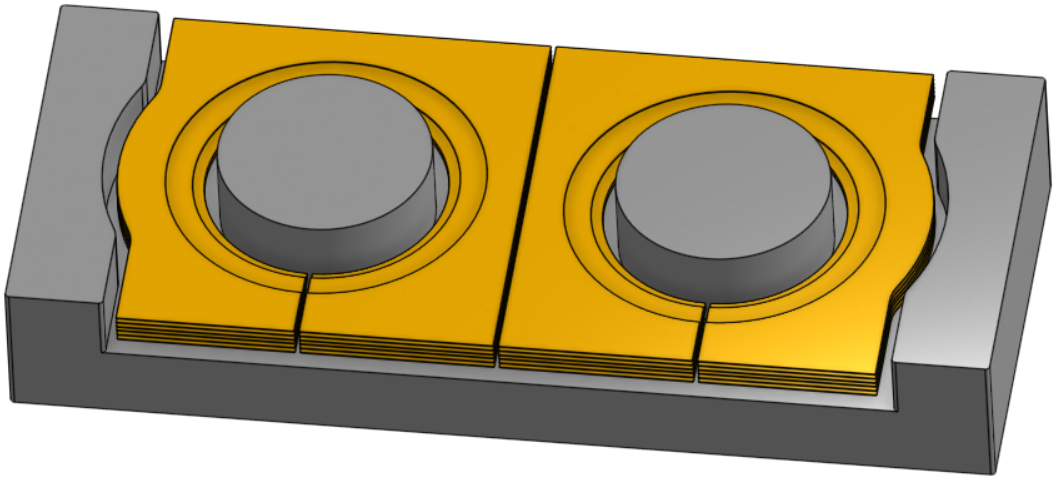
\includegraphics[width=0.6\columnwidth]{../figures/Four-Pole-3d.png}
  \caption{Final design of the four-pole inductor; top-piece not shown.}
  \label{fig:Four-Pole-3d}
\end{figure}

\section{Experimental prototype}
\begin{figure}
  \centering
  \includegraphics[page=2, trim = 0cm 0cm 3cm 0cm, clip, width=0.8\columnwidth]{../figures/IPEC_Figures_PowerPoint.pdf}
  \caption{Fully assembled prototype (without heatspreader).  The converter area shown in orange is 45 x 29 x \qty{9.5}{\mm}. Outside of this area only the connectors for power and programming are placed as well as a protection diode and the programming resistors.}
  \label{fig:PrototypePicture}
\end{figure}

\begin{table}
  \caption{Overview of the main hardware components.}
  \label{tab:Hardware}
  \centering
  \begin{tblr}{
      colspec={ll},
      row{1}={font=\bfseries},
      row{even}={bg=gray!10},
    }
    Component & Part \\
    \toprule
    $\mathrm C_\mathrm{in}$         & 44x \qty{2.2}{\uF} \qty{100}{\V} X7R (\qty{20}{\uF} at \qty{48}{\V})  \\
    $\mathrm C_\mathrm{out}$        & 16x \qty{2.2}{\uF} \qty{100}{\V} X7R (\qty{33}{\uF} at \qty{12}{\V}) \\
    GaN-FETs          & Infineon IGC025S08S1            \\
    Gate Driver       & Analog Devices LT8418           \\
    Microcontroller   & Texas Instruments F280049C      \\
    Aux. Power Supply & Texas Instruments TPSM365R6     \\
    Current Sensor    & Allegro ACS37220                \\  
    \bottomrule
  \end{tblr}
\end{table}

The assembled prototype is shown in Fig. \ref{fig:PrototypePicture}. The boxed volume of just \qty{12.4}{\cubic\cm} results in a power density of \qty{80}{\kW\per\liter} (\qty{1300}{\W\per\cubic\inch}). It's main hardware components are listed in table \ref{tab:Hardware}. Two parallel low side transistors per phase are used as the converter operates at a low duty cycle. To minimize the stray inductance, the decoupling capacitors for the half-bridges are connected to the devices with a so-called vertical power-loop layout which uses the first inner layer as a return path \cite{reuschUnderstandingEffectPCB2014}. In contrast to other designs, the large onboard capacitance allows the converter to operate without any additional off-board capacitance. \par
The converter operates over the entire power range as expected. The efficiency is shown in Fig. \ref{fig:Efficiency} which reaches its maximum of \qty{96.3}{\percent} at around \qty{550}{\W} putting it in the same range as comparable LLC designs \cite{caiOptimalDesignMegahertz2020, ahmedLowLossIntegratedInductor2020}. As expected, the efficiency significantly drops for each frequency once a certain power is exceeded. This is caused by the operation in \ac{tcm}: The leg-current ripple is proportional to the switching frequency and to achieve soft-switching, a certain negative current is required prior to the turn-off of the low-side switch. Otherwise, the voltage at the switching node will not rise fast enough to yield soft-switching. As the output current rises, the negative current rises and at some point, soft-switching is lost. To use the converter in a real application, a variable switching frequency is required. The expected resulting efficiency curve is indicated in Fig. \ref{fig:Efficiency}.

\begin{figure}
  \centering
  \input{../figures/Efficiency_48V_TDK.tikz}
  \caption{Efficiency of the prototype for $\sbl{Vin}=\qty{48}{\V}$ and $D=0.25$.}
  \label{fig:Efficiency}
\end{figure}

\section{Conclusion}
This paper introduced a novel, negatively coupled, single turn inductor which enables very high power density and efficiency in a two-phase buck converter for \qty{48}{\V} to \qty{12}{\V} conversion. The effects of positive and negative coupling were evaluated in detail. It was shown that even though negative coupling exhibits higher leg and output current ripple, it allows a much more compact construction due to the lower DC flux. A dual air gap and an optimized winding geometry were introduced which reduce losses by \qty{30}{\percent}. Following the comparison of four different inductor geometries, the best design was implemented in an experimental prototype which achieves a power density of \qty{80}{\kW\per\l} (\qty{1300}{\W\per\cubic\inch}) for \qty{1}{\kW} and a peak efficiency of \qty{96.3}{\percent}, demonstrating the potential of the inductor. \par
The final paper will add a more detailed analysis of the losses, comparing the different sources of losses in simulation with measurements from the prototype. More detailed measurements will also be presented, showing efficiency for a fixed conversion ratio instead of fixed duty cycle as well as efficiency in boost-mode. 

\bibliographystyle{IEEEtranNDoi}
\bibliography{Paper_Bibliography}

\end{document}

% https://ipec2026.org/regular-session/ 

% The extended summary should clearly define the salient concepts
% and novel features of the work. Be sure to mention past or
% previous works to distinguish your originality from them. The
% extended summary should be up to 4 pages except Reference,